\documentclass[border=10pt]{standalone}
\usepackage[svgnames]{xcolor}
\usepackage{amsmath}
\usepackage{pgfplots}
\pgfplotsset{compat=newest}
\usepackage[sfdefault]{FiraSans}
\usepackage{FiraMono}
\renewcommand*\familydefault{\sfdefault}
\begin{document}
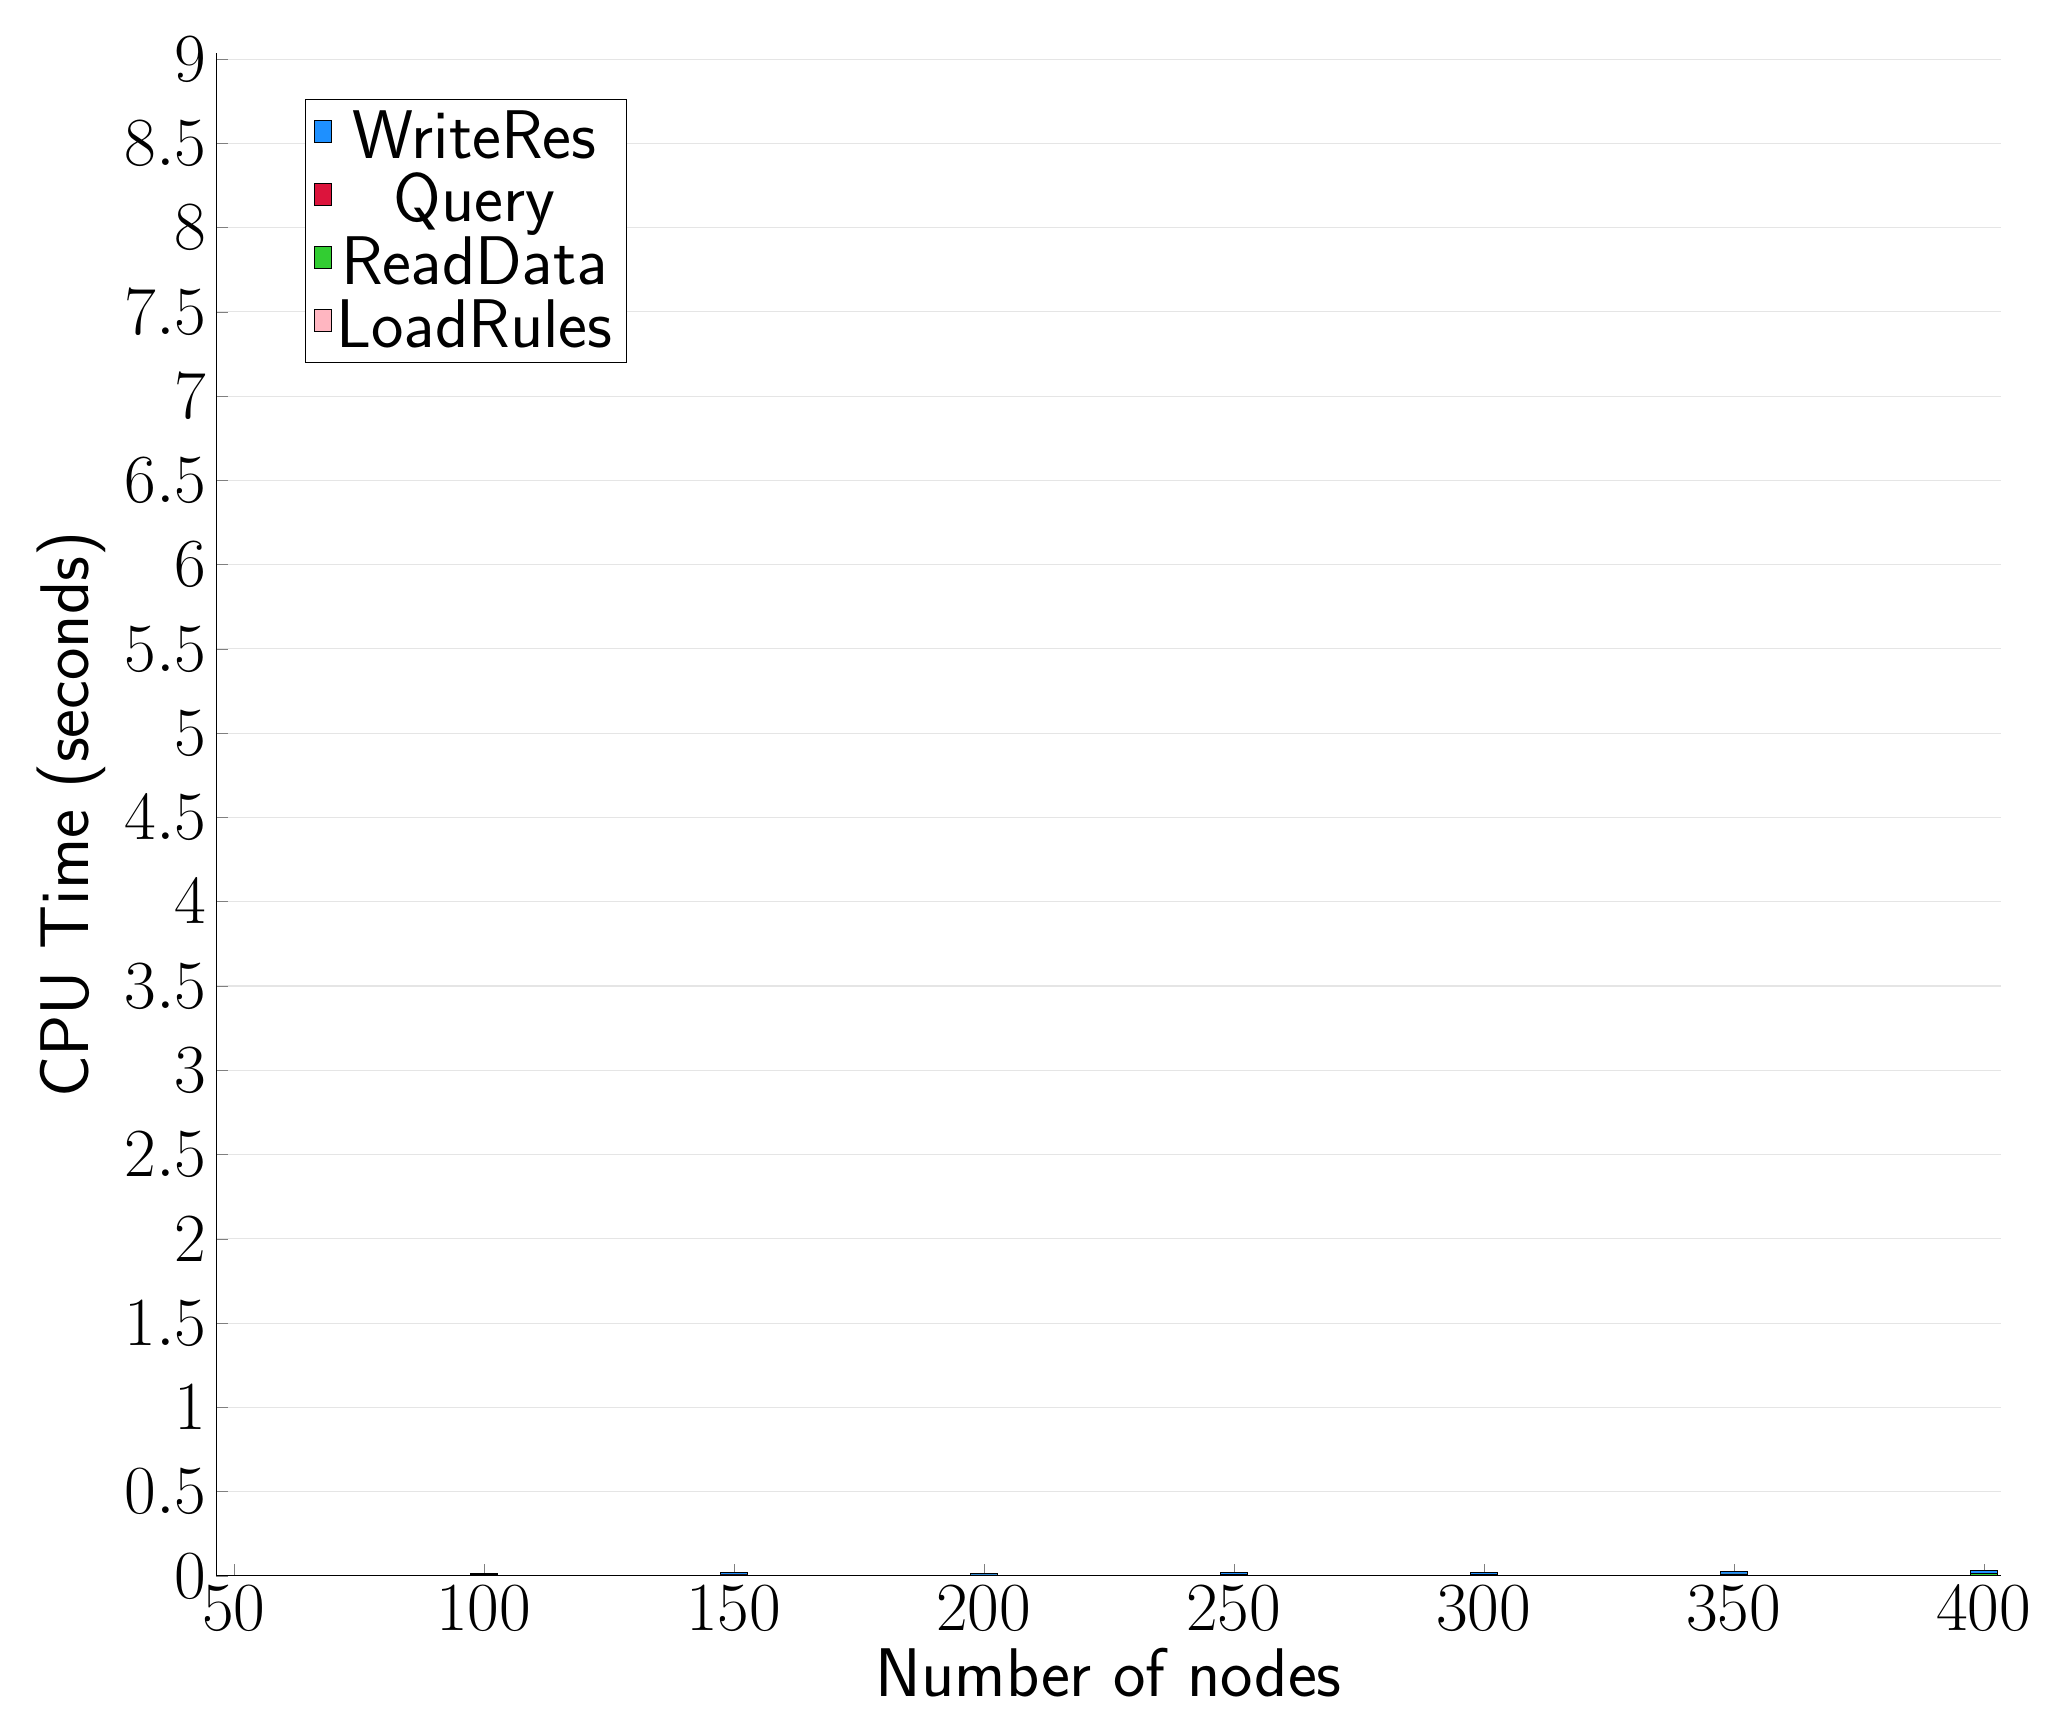
\begin{tikzpicture}
\begin{axis}[
   ybar stacked,
   width=2\textwidth,
   bar width=0.35cm,
   ymajorgrids, tick align=inside,
   major grid style={draw=gray!20},
   xtick=data,
   ymin=0, ymax=9.033333333830038,
   axis x line*=bottom,
   axis y line*=left,
   enlarge x limits=0.01,
   legend style={
       at={(0.23, 0.97)},
       anchor=north east,
       legend columns=1,
       font=\Huge,
   },
   ylabel={CPU Time (seconds)},
   xlabel={Number of nodes},
   label style={font=\Huge},
   tick label style={font=\Huge},
]
\addlegendimage{fill=DodgerBlue, draw=black, line width=0.2pt}
\addlegendentry{WriteRes}
\addlegendimage{fill=Crimson, draw=black, line width=0.2pt}
\addlegendentry{Query}
\addlegendimage{fill=LimeGreen, draw=black, line width=0.2pt}
\addlegendentry{ReadData}
\addlegendimage{fill=LightPink, draw=black, line width=0.2pt}
\addlegendentry{LoadRules}
\addplot +[fill=LightPink, draw=black, line width=0.2pt] coordinates {
(50, 0.0033996666666666667)
(100, 0.005092666666666666)
(150, 0.006569333333333333)
(200, 0.0031886666666666665)
(250, 0.004979666666666667)
(300, 0.003637999999999999)
(350, 0.005184999999999997)
(400, 0.00493166666666667)
};
\addplot +[fill=LimeGreen, draw=black, line width=0.2pt] coordinates {
(50, 0.0006920000000000042)
(100, 0.0031666666666666666)
(150, 0.004001666666666667)
(200, 0.0028580000000000046)
(250, 0.005025000000000007)
(300, 0.004421999999999996)
(350, 0.00715466666666667)
(400, 0.007785333333333334)
};
\addplot +[fill=Crimson, draw=black, line width=0.2pt] coordinates {
(50, 1.59999999999975e-05)
(100, 6.533333333333159e-05)
(150, 9.233333333333317e-05)
(200, 9.733333333332904e-05)
(250, 8.299999999999513e-05)
(300, 8.866666666666744e-05)
(350, 0.00012399999999999667)
(400, 0.00013799999999999902)
};
\addplot +[fill=DodgerBlue, draw=black, line width=0.2pt] coordinates {
(50, 0.0009703333333333357)
(100, 0.005445666666666668)
(150, 0.007921333333333338)
(200, 0.010418666666666672)
(250, 0.011607000000000004)
(300, 0.010902666666666666)
(350, 0.016127000000000002)
(400, 0.020295333333333332)
};
\end{axis}
\end{tikzpicture}

\end{document}
